\subsection{Results}
\label{sec:results}

\subsubsection{Prediction of valence and arousal}

The primary seven-feature model produced a modest improvement for arousal and no improvement for valence in the provisional sample. Table~\ref{tab:performance} reports pooled out-of-fold errors, so every evaluated prediction comes from a model that excluded the corresponding artist-credit group. The predictions are evaluated on the supplied numerical label scale. No primary ridge predictions fell outside $[0,1]$.

\begin{table}[ht]
\centering
\caption{Primary grouped evaluation on 92 provisional dance-style excerpts. Lower RMSE and MAE indicate smaller errors. The responses are evaluated separately.}
\label{tab:performance}
\begin{tabular}{llrrr}
\toprule
Response & Method & RMSE & MAE & $R^2$ \\
\midrule
Valence & Training mean & 0.1828 & 0.1612 & -0.007 \\
Valence & Ordinary least squares & 0.1935 & 0.1637 & -0.128 \\
Valence & Ridge & 0.1873 & 0.1651 & -0.057 \\
Arousal & Training mean & 0.0992 & 0.0726 & -0.001 \\
Arousal & Ordinary least squares & 0.0945 & 0.0690 & 0.090 \\
Arousal & Ridge & 0.0931 & 0.0682 & 0.118 \\
\bottomrule
\end{tabular}
\end{table}

For arousal, ridge reduced RMSE from 0.0992 for the training-mean baseline to 0.0931, a relative reduction of approximately 6.2\%. Its out-of-fold $R^2$ was 0.118. For valence, ridge RMSE was 0.1873, compared with 0.1828 for the baseline, and $R^2$ was -0.057. Thus the measured acoustic summaries provided some useful information about activation under this evaluation, but they did not improve the prediction of emotional positivity.

\begin{figure}[ht]
\centering
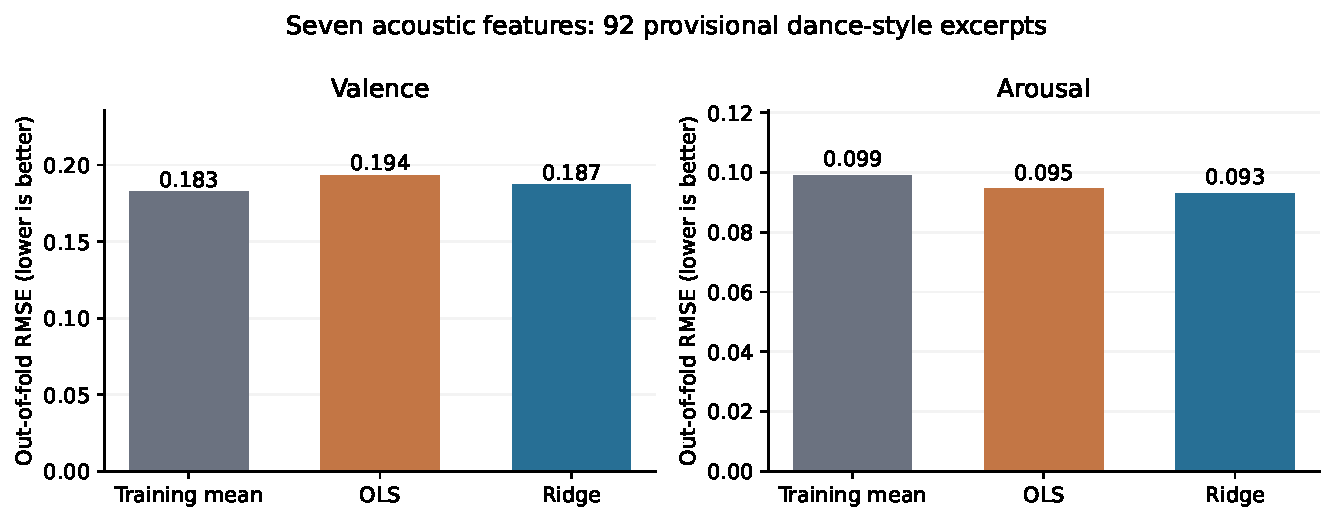
\includegraphics[width=\linewidth]{figures/01_prediction_error.pdf}
\caption{Out-of-fold prediction errors for the training-mean baseline, ordinary least squares, and ridge regression. Each panel begins at zero; the panels have different vertical scales.}
\label{fig:error}
\end{figure}

The numerical error magnitudes should not be compared directly across responses because the supplied arousal scores vary less than the valence scores. Baseline comparisons and $R^2$ are more informative for this purpose. Ordinary least squares also improved on the arousal baseline but had larger error than ridge. Both regression approaches performed worse than the baseline for valence.

\begin{figure}[ht]
\centering
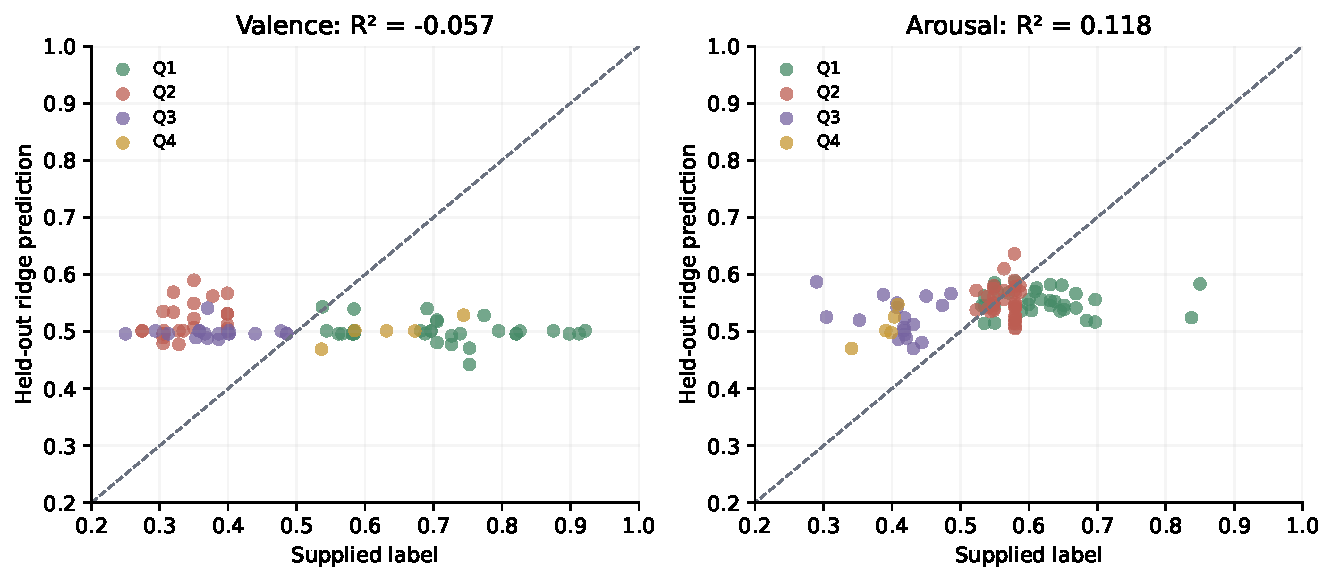
\includegraphics[width=\linewidth]{figures/02_observed_predicted.pdf}
\caption{Supplied labels versus held-out ridge predictions. The dashed line represents perfect prediction. Colors identify the supplied mood quadrants. Points illustrate the restricted range of many predictions, especially for valence.}
\label{fig:predictions}
\end{figure}

The valence predictions are concentrated near the middle of the observed label range. Inner validation selected the largest penalty, $\lambda=10^4$, in three of the five outer folds, leaving these fits close to their training means. This supports a limited interpretation: the seven predictors did not provide sufficiently useful valence information to justify a more flexible linear fit in those folds. It does not imply that valence cannot be predicted from music, since harmony, melodic characteristics, lyrics, and richer representations are absent from this model.

\subsubsection{Which measurements provide useful information?}

Spectral brightness and positive spectral flux had positive arousal coefficients in all five outer models. Their coefficient ranges are shown in Figure~\ref{fig:coefficients}. These are fitted associations conditional on the other measurements. Since predictors are correlated and the penalty changes across folds, coefficient magnitude alone is not a complete measure of predictive usefulness.

\begin{figure}[ht]
\centering
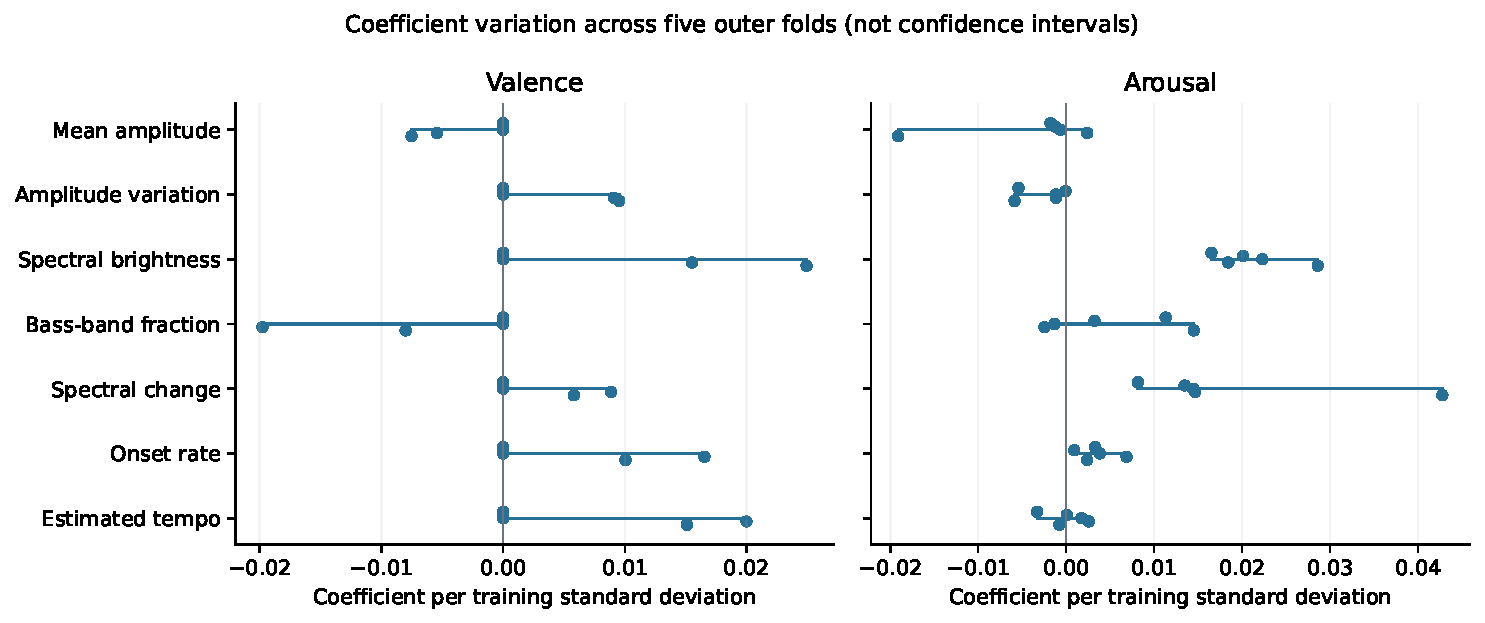
\includegraphics[width=\linewidth]{figures/03_fold_coefficients.pdf}
\caption{Standardized coefficients from the five outer ridge fits. Each dot is a fold-specific estimate, and the line shows the observed range. These ranges describe split variation and are not confidence intervals.}
\label{fig:coefficients}
\end{figure}

We therefore also removed each feature family and refitted and retuned the remaining model. Table~\ref{tab:ablation} reports the aggregate held-out error changes. Omitting brightness and spectral change increased arousal RMSE by approximately $0.0074$, from about $0.0931$ to $0.1004$. It worsened arousal prediction in each outer fold. This was the clearest family-removal effect in the primary analysis. Omitting bass-band content produced a smaller aggregate increase of about $0.0014$, with mixed fold-level effects. Omitting amplitude or rhythm slightly lowered aggregate arousal error in this split. For valence, all aggregate changes were small and the full model itself did not outperform the baseline.

\begin{table}[ht]
\centering
\caption{Change in pooled out-of-fold RMSE after omitting a feature family and retuning. Positive values mean worse prediction than the full ridge model.}
\label{tab:ablation}
\begin{tabular}{lrr}
\toprule
Omitted family & Valence change & Arousal change \\
\midrule
Amplitude & +0.0003 & -0.0005 \\
Rhythm & -0.0013 & -0.0010 \\
Brightness/change & -0.0012 & +0.0074 \\
Bass band & +0.0007 & +0.0014 \\
\bottomrule
\end{tabular}
\end{table}

\begin{figure}[ht]
\centering
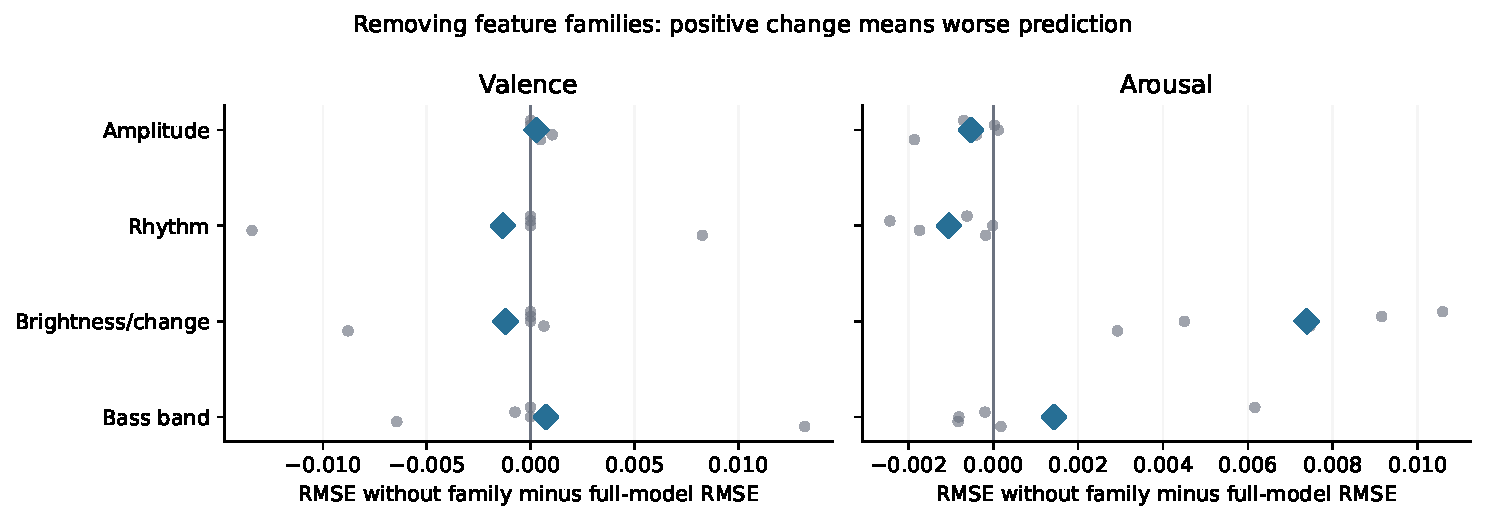
\includegraphics[width=\linewidth]{figures/04_feature_family_ablation.pdf}
\caption{Feature-family removal results. Diamonds show changes in aggregate RMSE; smaller dots show changes within individual outer folds. The fold results do not form independent samples.}
\label{fig:ablation}
\end{figure}

The descriptive correlations provide a compatible, less controlled view. Spectral centroid correlated with arousal at approximately $0.481$, and positive spectral flux at approximately $0.371$. Estimated tempo had an arousal correlation close to zero, approximately $-0.003$. These are excerpt-level correlations in the selected sample, without adjustment for genre composition or artist identity. They should not be interpreted as evidence that changing tempo has no effect on emotion. Beat-tracking errors, production choices, and the limited sample can all affect this relationship.

\subsubsection{Sensitivity to artist-credit group splits}

Across ten grouped split seeds, ridge improved arousal RMSE relative to the corresponding training-mean baseline in all ten evaluations. Arousal $R^2$ ranged from -0.066 to 0.176. Valence ridge RMSE was worse than its baseline in nine of the ten evaluations, and its $R^2$ ranged from -0.115 to -0.013. The overall direction is therefore more stable than the exact score, particularly for arousal. These ranges describe sensitivity to overlapping partitions of the same 92 observations and are not independent-sample confidence intervals.

An additional summary weights each artist-credit group equally by averaging squared errors within a group and then across groups. In the primary split, equal-group arousal RMSE was approximately $0.1011$ for ridge and $0.1074$ for the baseline. Equal-group valence RMSE was approximately $0.1941$ for ridge and $0.1903$ for the baseline. This check preserved the direction of the main comparison while reducing the influence of artists with several excerpts.

\subsubsection{Temporal variation and EDM structure}

The additional temporal analysis examines a musically important question: whether the way the sound changes within an excerpt adds information beyond its average characteristics. The twelve-feature model adds the three time slopes and two adjacent-bin changes defined in Section~\ref{sec:model}. It retains the same static responses and the same outer grouping.

In the primary split, the temporal model obtained valence RMSE 0.1863 and $R^2=-0.045$, and arousal RMSE 0.0926 and $R^2=0.126$. These errors are slightly smaller than those of the seven-feature model. Across ten split seeds, however, the temporal extension improved on the seven-feature model in 3 evaluations for valence and 8 for arousal. The direction varied between partitions. We therefore found no consistent evidence that this particular set of coarse temporal descriptors adds substantial predictive value. This extension was introduced after examining the primary analysis and should be treated as exploratory.

\begin{figure}[ht]
\centering
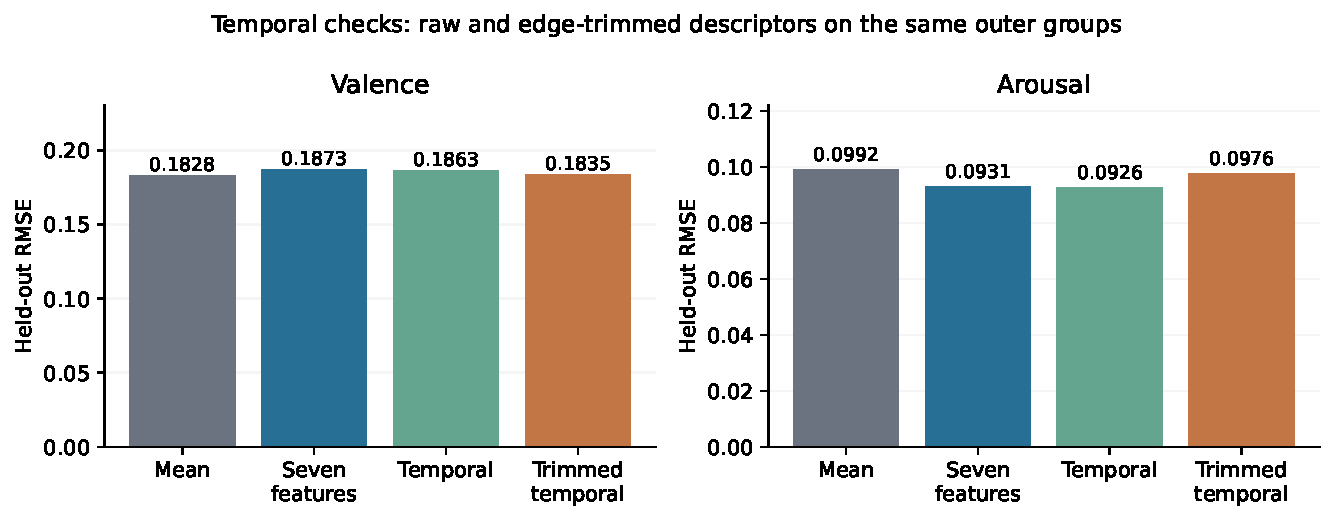
\includegraphics[width=\linewidth]{figures/08_temporal_model_comparison.pdf}
\caption{Primary-split errors for the baseline, seven-feature model, raw temporal extension, and edge-trimmed temporal diagnostic. The temporal checks are exploratory; small improvements were not consistently reproduced across group assignments.}
\label{fig:temporalcomparison}
\end{figure}

Figure~\ref{fig:profiles} shows two examples selected by the largest adjacent-bin increase in amplitude, independently of prediction accuracy. The excerpt from The Prodigy's \emph{We Are the Ruffest} had a maximum increase of approximately $24.34$ dB between adjacent bins, while Fennesz's \emph{Transit} had an increase of approximately $17.33$ dB. These values compare averaged amplitudes in adjacent bins of roughly three seconds. They can be affected by pauses, fades, editing, and other acoustic changes. They are not validated measurements of a drop's intensity.

\begin{figure}[ht]
\centering
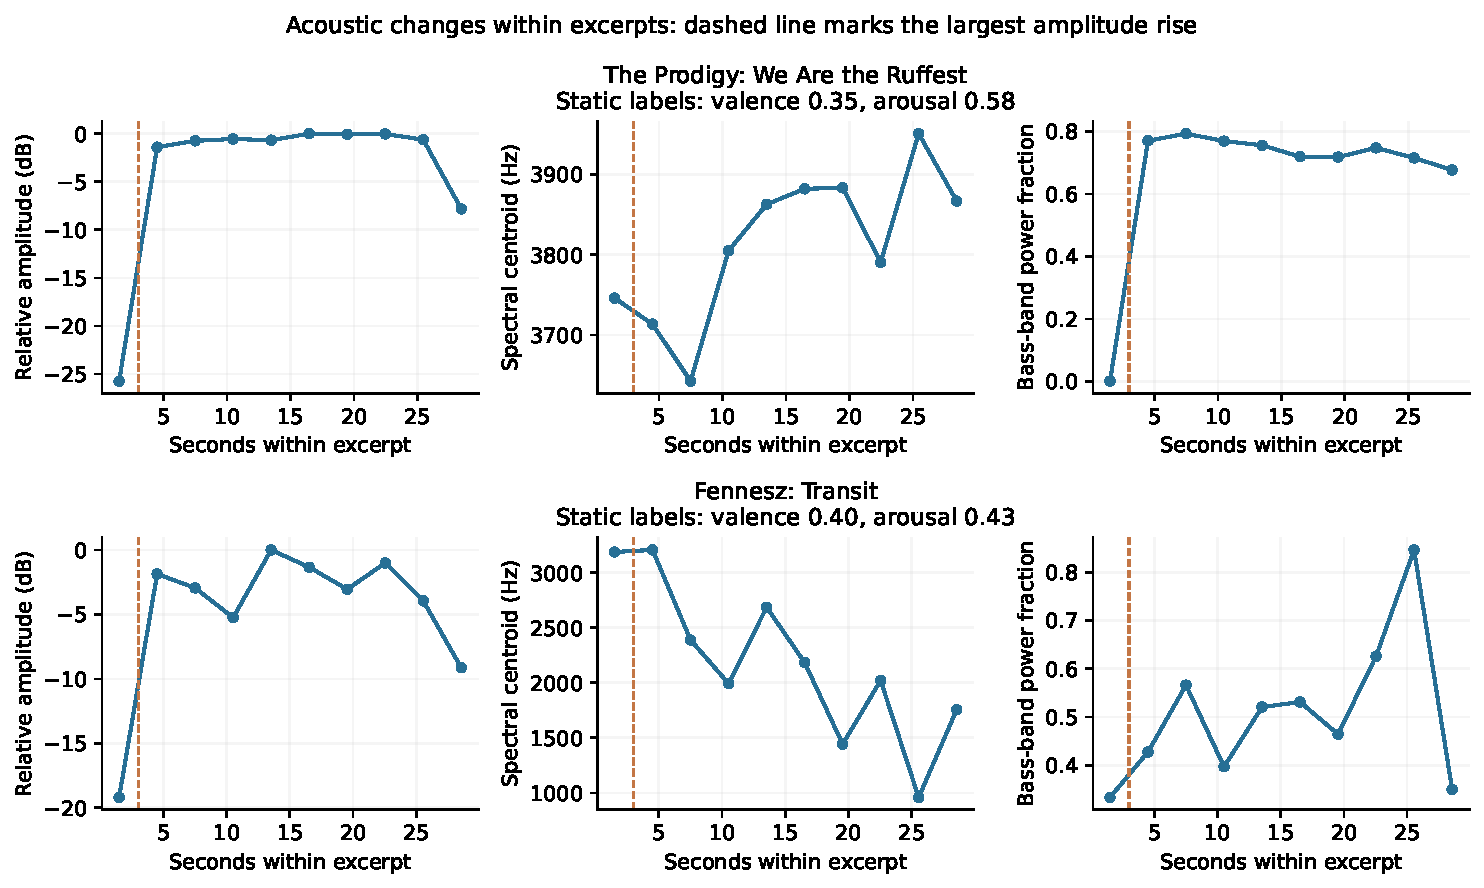
\includegraphics[width=\linewidth]{figures/07_temporal_profiles.pdf}
\caption{Ten-bin acoustic profiles for two descriptively selected examples. The dashed line marks the boundary with the largest increase in bin-average amplitude. Its position does not constitute a confirmed buildup or drop boundary. Each recording has one supplied static emotion pair, not separate emotion labels for the plotted bins.}
\label{fig:profiles}
\end{figure}

To connect these measurements to musical structure, Table~\ref{tab:sections} gives operational cues for later manual annotation. These cues guide listening and feature comparisons; they are not outputs of a trained section detector. A meaningful buildup-to-drop analysis requires the preceding context and a confirmed transition. A 30-second excerpt may contain only part of a section or begin after the transition has occurred.

\begin{table}[ht]
\centering
\caption{Proposed listening cues and measurements for annotated case-study sections. These are analysis criteria, not section labels assigned to the 92 excerpts.}
\label{tab:sections}
\begin{tabular}{p{0.15\linewidth}p{0.35\linewidth}p{0.38\linewidth}}
\toprule
Section & Listening cue to review & Measurement to compare \\
\midrule
Breakdown & Reduced rhythmic activity relative to neighboring sections & Onset rate, amplitude, and bass-band content \\
Buildup & Accumulation of rhythmic or spectral activity before a transition & Time slopes of onset rate and brightness \\
Drop & Re-entry or change in the main rhythmic and low-frequency texture & Changes relative to the preceding buildup \\
Core & A comparatively sustained groove or texture & Feature levels and within-section variation \\
\bottomrule
\end{tabular}
\end{table}

The case-study code can calculate features from independently annotated sections and express the difference between their model-input predictions as a sum of feature changes. A valid listening claim about emotional change would additionally require section-level emotion annotations. Consequently, the present results concern acoustic variation associated with an overall mood score. We have not established how perceived sadness changes from breakdown to buildup to drop.

The position of the largest amplitude change raised a further concern. In 69 of the 92 excerpts, the maximum adjacent-bin amplitude rise occurred after the first bin, near three seconds into the clip. This concentration near the beginning suggests that excerpt boundaries, fades, or editing may influence the descriptor. It would therefore be misleading to count these changes as identified drops.

As a post-hoc diagnostic, we recomputed the five temporal descriptors after omitting the first and last bins. The primary-split trimmed model had valence RMSE 0.1835 and arousal RMSE 0.0976. It still failed to outperform the valence baseline, and its arousal error was larger than that of the original seven-feature model. These results reinforce the need to separate acoustic change from verified musical structure. The diagnostic was motivated by the boundary audit and is not an independently prespecified test.

\subsubsection{Interpretation and limitations}

For a general audience, the primary result can be stated as follows: characteristics of sound texture helped us estimate how activated a recording was, while these initial measurements did not reliably distinguish positive from negative mood. The separation of valence and arousal is useful because intensity and emotional positivity need not have the same acoustic relationships. The evidence is strongest for the brightness/change feature family within this model and sample.

Several limitations shape that interpretation. First, the 92 candidates include dance-pop, experimental, and crossover material, and their final EDM membership has not been manually verified. Second, Q4 contains only five excerpts, and the response distributions do not represent mood prevalence in all EDM. Third, the labels come from MERGE's tag-based annotation process. Fourth, grouping complete artist credits reduces one source of leakage but does not resolve aliases, overlapping collaborators, or all possible related recordings. Fifth, the model is linear and omits harmony, lyrical meaning, detailed melody, and isolated-source features. Sixth, ten temporal bins cannot replace annotated full-song structure. The exploratory results can guide the next phase, but they do not justify a universal rule about what makes EDM sad.
